% Table generated by Excel2LaTeX from sheet 'Tabelle1'

\begin{longtabu}to\textwidth{X[1,c]X[4,c]X[6,c]X[6,c]X[4,c]X[1,c]}
\captionsetup{tablewithin = chapter}
\captionsetup{font=small, labelfont=bf}
\captionabove[{Zerlegung der $^{31}$P Verschiebung in Orbitalbeiträge}]{\ac{mo} Beiträge zur $^{31}$P Verschiebung. Orbitale die weniger als \unit[1]{ppm} beitragen wurden nicht mit aufgenommen. Die am meisten beitragenden Orbitale wurden mit einem X gekennzeichnet und sind in Abbildung \ref{abb:modec} gezeigt. Zur Reduktion der Probleme, die durch die Eichinvarianz auftreten, wurde das Molekül so verschoben, dass das Phosphoratom im Ursprung liegt.\label{tab:cvhzerlegung}}\\
    \hline
    \hline
    \ac{mo} & Energie / eV & diamagnetischer Beitrag & paramagnetischer Beitrag & gesamt &  \\
    \hline
    %
  \endfirsthead % Erster Kopf zu Ende
  \multicolumn{6}{l}{\ldots Fortsetzung}\\
  \ac{mo} & Energie / eV & diamagnetischer Beitrag & paramagnetischer Beitrag & gesamt &  \\
  \hline
  \endhead
%
  \multicolumn{6}{r}{wird fortgesetzt \ldots}
  \endfoot
  \endlastfoot
%	\endfirsthead % Erster Kopf zu Ende
	%  Definition des Tabellenkopfes auf den folgenden Seiten
%	\caption{Fortsetzung}\\%
%	\ac{mo} & Energie / eV & diamagnetischer Beitrag & paramagnetischer Beitrag & gesamt &  \\
%	\hline
%	\endhead % Zweiter Kopf ist zu Ende
%	Weiter auf der n{\"a}chste Seite\\
%	\endfoot
%	\hline
%	Vor dem endlastfoot: Tabelle zu Ende \\
%\endlastfoot
% Ab hier kommt der Inhalt der Tabelle
    4     & -2075.219 & 517.191836 & -0.0045397 & 517.187296 & X \\
    56    & -170.577 & 99.4654758 & 0.09861722 & 99.564093 & X \\
    59    & -122.029 & 92.6938755 & 34.7117998 & 127.405675 & X \\
    60    & -121.991 & 95.9498071 & -4.87383336 & 91.0759738 & X \\
    61    & -121.983 & 95.8039826 & -5.30359114 & 90.5003915 & X \\
    68    & -25.662 & 0.53404716 & 1.3546215 & 1.88866866 &  \\
    69    & -23.408 & -0.09814514 & 3.16604807 & 3.06790293 &  \\
    70    & -21.627 & 0.01959928 & 1.78702756 & 1.80662684 &  \\
    71    & -21.234 & 0.02197222 & 1.95831192 & 1.98028413 &  \\
    72    & -19.775 & -0.01793399 & 2.4592444 & 2.44131041 &  \\
    73    & -19.633 & 0.24167534 & 6.54078556 & 6.78246089 &  \\
    74    & -19.57 & -0.02172001 & 1.09340645 & 1.07168644 &  \\
    76    & -19.473 & 0.09386996 & 2.11593358 & 2.20980355 &  \\
    77    & -19.446 & 0.08714956 & 1.87050869 & 1.95765824 &  \\
    78    & -19.368 & 0.13194102 & 2.12303904 & 2.25498006 &  \\
    79    & -19.362 & 0.49287261 & -4.45535897 & -3.96248637 &  \\
    80    & -19.357 & 0.18579217 & 1.20863043 & 1.3944226 &  \\
    81    & -19.202 & -0.00201103 & 1.5980115 & 1.59600048 &  \\
    93    & -17.403 & 0.01353283 & 2.14047301 & 2.15400584 &  \\
    94    & -17.354 & -0.01692121 & 1.55183281 & 1.53491159 &  \\
    95    & -16.901 & -0.01320885 & 1.1277965 & 1.11458766 &  \\
    96    & -16.814 & 0.01229753 & 1.00358603 & 1.01588356 &  \\
    97    & -16.764 & -0.01172257 & 1.21713482 & 1.20541225 &  \\
    98    & -16.437 & 0.02021503 & 1.63625805 & 1.65647307 &  \\
    99    & -16.434 & 0.06779826 & 1.45607779 & 1.52387604 &  \\
    100   & -16.374 & 0.06596182 & 1.75989832 & 1.82586014 &  \\
    101   & -16.303 & 0.03007284 & 1.32661045 & 1.35668329 &  \\
    102   & -16.29 & 0.01787841 & 1.52573046 & 1.54360887 &  \\
    103   & -16.268 & 0.02568144 & 1.42316584 & 1.44884728 &  \\
    104   & -16.195 & 0.01887398 & 1.47227302 & 1.491147 &  \\
    105   & -16.142 & 0.02095796 & 1.50018399 & 1.52114195 &  \\
    106   & -15.952 & 0.04972872 & 1.53983104 & 1.58955976 &  \\
    107   & -15.68 & 6.94363928 & 0.69097726 & 7.63461654 &  \\
    108   & -15.051 & 3.05882791 & 2.36501176 & 5.42383967 &  \\
    112   & -13.518 & 0.81685183 & 0.74118574 & 1.55803757 &  \\
    113   & -13.116 & 0.16457604 & 1.78343911 & 1.94801516 &  \\
    114   & -12.945 & 1.25055266 & -0.04451094 & 1.20604171 &  \\
    115   & -12.836 & 0.16214427 & -1.90735225 & -1.74520798 &  \\
    116   & -12.561 & 0.1415055 & 1.15076135 & 1.29226684 &  \\
    117   & -12.556 & 3.78081903 & 5.91381542 & 9.69463445 &  \\
    118   & -12.483 & 0.12979966 & 1.07317233 & 1.20297198 &  \\
    119   & -12.48 & 0.32351403 & 1.25053545 & 1.57404948 &  \\
    120   & -12.129 & 0.54584208 & 1.34398803 & 1.88983012 &  \\
    121   & -11.93 & 0.09249229 & 3.24272225 & 3.33521454 &  \\
    122   & -11.276 & 0.44510731 & -16.7759414 & -16.3308341 &  \\
    123   & -11.273 & 0.33385082 & -9.0936797 & -8.75982889 &  \\
    124   & -11.139 & 0.17615005 & -1.64865544 & -1.47250539 &  \\
    125   & -11.108 & 0.51873119 & -5.03044193 & -4.51171074 &  \\
    126   & -10.787 & 0.03447635 & -1.2173175 & -1.18284116 &  \\
    127   & -10.726 & 0.06770143 & 1.40499911 & 1.47270054 &  \\
    128   & -10.662 & 0.06156794 & 2.91941845 & 2.9809864 &  \\
    134   & -10.281 & 0.04467939 & 1.25376753 & 1.29844691 &  \\
    136   & -10.209 & 0.48598321 & -9.11261675 & -8.62663355 &  \\
    137   & -10.185 & 0.07291205 & 1.55274159 & 1.62565365 &  \\
    138   & -10.144 & 0.07830575 & 1.02481432 & 1.10312007 &  \\
    141   & -10.066 & 0.1364759 & -1.83547857 & -1.69900267 &  \\
    143   & -9.962 & 0.18119511 & -11.9269724 & -11.7457772 &  \\
    145   & -9.901 & 0.54552586 & -6.83025033 & -6.28472447 &  \\
    146   & -9.893 & 0.01054856 & 1.15279966 & 1.16334822 &  \\
    148   & -9.795 & 0.04937586 & -1.11751888 & -1.06814303 &  \\
    149   & -9.771 & 1.57970367 & -35.43946 & -33.8597563 &  \\
    150   & -9.749 & 1.05654025 & -36.5240686 & -35.4675283 &  \\
    151   & -9.616 & 0.14242252 & -3.05971013 & -2.91728761 &  \\
    152   & -9.603 & 0.54286829 & -14.0900846 & -13.5472163 &  \\
    154   & -9.078 & 0.45679481 & -6.25269617 & -5.79590137 &  \\
    155   & -9.022 & 0.30521796 & -2.89719583 & -2.59197787 &  \\
    157   & -8.915 & 0.3317604 & -12.0465755 & -11.7148151 &  \\
    158   & -8.894 & 0.03499415 & -2.23272019 & -2.19772604 &  \\
    159   & -8.852 & 0.12790544 & -1.78054627 & -1.65264083 &  \\
    160   & -8.836 & 0.11569778 & -4.18203675 & -4.06633897 &  \\
    161   & -8.821 & 0.22141616 & -2.88978294 & -2.66836679 &  \\
    163   & -8.685 & -0.04341331 & -1.06858108 & -1.11199439 &  \\
    164   & -8.613 & -0.03929554 & -1.37310952 & -1.41240506 &  \\
    165   & -8.567 & 0.49516778 & -14.9968916 & -14.5017238 &  \\
    166   & -8.416 & 0.03588159 & -2.28427077 & -2.24838919 &  \\
    167   & -8.368 & 0.00248013 & -2.06308801 & -2.06060789 &  \\
    168   & -8.331 & 0.03514653 & -2.25281836 & -2.21767183 &  \\
    169   & -8.325 & 0.03804272 & -1.083833 & -1.04579028 &  \\
    170   & -8.287 & 0.01021177 & -2.13399407 & -2.1237823 &  \\
    171   & -8.262 & -0.01101696 & -1.80433784 & -1.8153548 &  \\
    172   & -8.251 & 0.03656101 & -2.5156817 & -2.47912069 &  \\
    173   & -8.164 & 0.03218817 & -1.9596398 & -1.92745163 &  \\
    174   & -8.159 & 0.01339373 & -1.20803182 & -1.1946381 &  \\
    175   & -8.024 & 0.27091016 & -4.46817721 & -4.19726705 &  \\
    176   & -7.651 & 0.16272505 & -5.41820816 & -5.25548311 &  \\
    177   & -7.511 & 0.58622111 & -28.1015327 & -27.5153116 &  \\
    178   & -7.498 & 0.0600034 & -2.75059261 & -2.69058921 &  \\
    179   & -7.436 & 0.03258139 & -3.8819416 & -3.8493602 &  \\
    180   & -7.357 & 0.04926782 & -3.68748232 & -3.63821451 &  \\
    181   & -7.31 & 1.39166476 & -39.4294645 & -38.0377997 &  \\
    182   & -7.282 & 0.04584765 & -2.46897227 & -2.42312462 &  \\
    183   & -7.154 & 1.64417751 & -46.0412125 & -44.397035 &  \\
    184   & -7.14 & 0.81407613 & -24.8477059 & -24.0336297 &  \\
    185   & -6.995 & 1.21851146 & -33.2754464 & -32.056935 &  \\
    186   & -6.93 & 1.92326147 & -41.6456079 & -39.7223464 &  \\
    187   & -6.52 & 0.96541333 & 2.86932743 & 3.83474076 &  \\
    188   & -6.399 & 0.13594597 & 1.04337865 & 1.17932463 &  \\
    189   & -6.079 & 0.38325442 & -10.3976843 & -10.0144298 &  \\
    191   & -6.027 & 0.02032565 & -3.14864368 & -3.12831803 &  \\
    192   & -5.516 & 0.19730284 & -22.6888381 & -22.4915353 &  \\
    193   & -5.214 & 7.32158116 & -75.1069516 & -67.7853704 & X \\
    194   & -5.099 & 6.68651778 & 4.86354126 & 11.550059 &  \\
    195   & -4.892 & 0.15622881 & -4.87733749 & -4.72110868 &  \\
    196   & -4.434 & 7.95638357 & -117.389691 & -109.433307 & X \\
    gesamt &       & 962.655788 & -581.846494 & 380.809294 &  \\
\end{longtabu}

\begin{figure}[ht!]
	\centering
	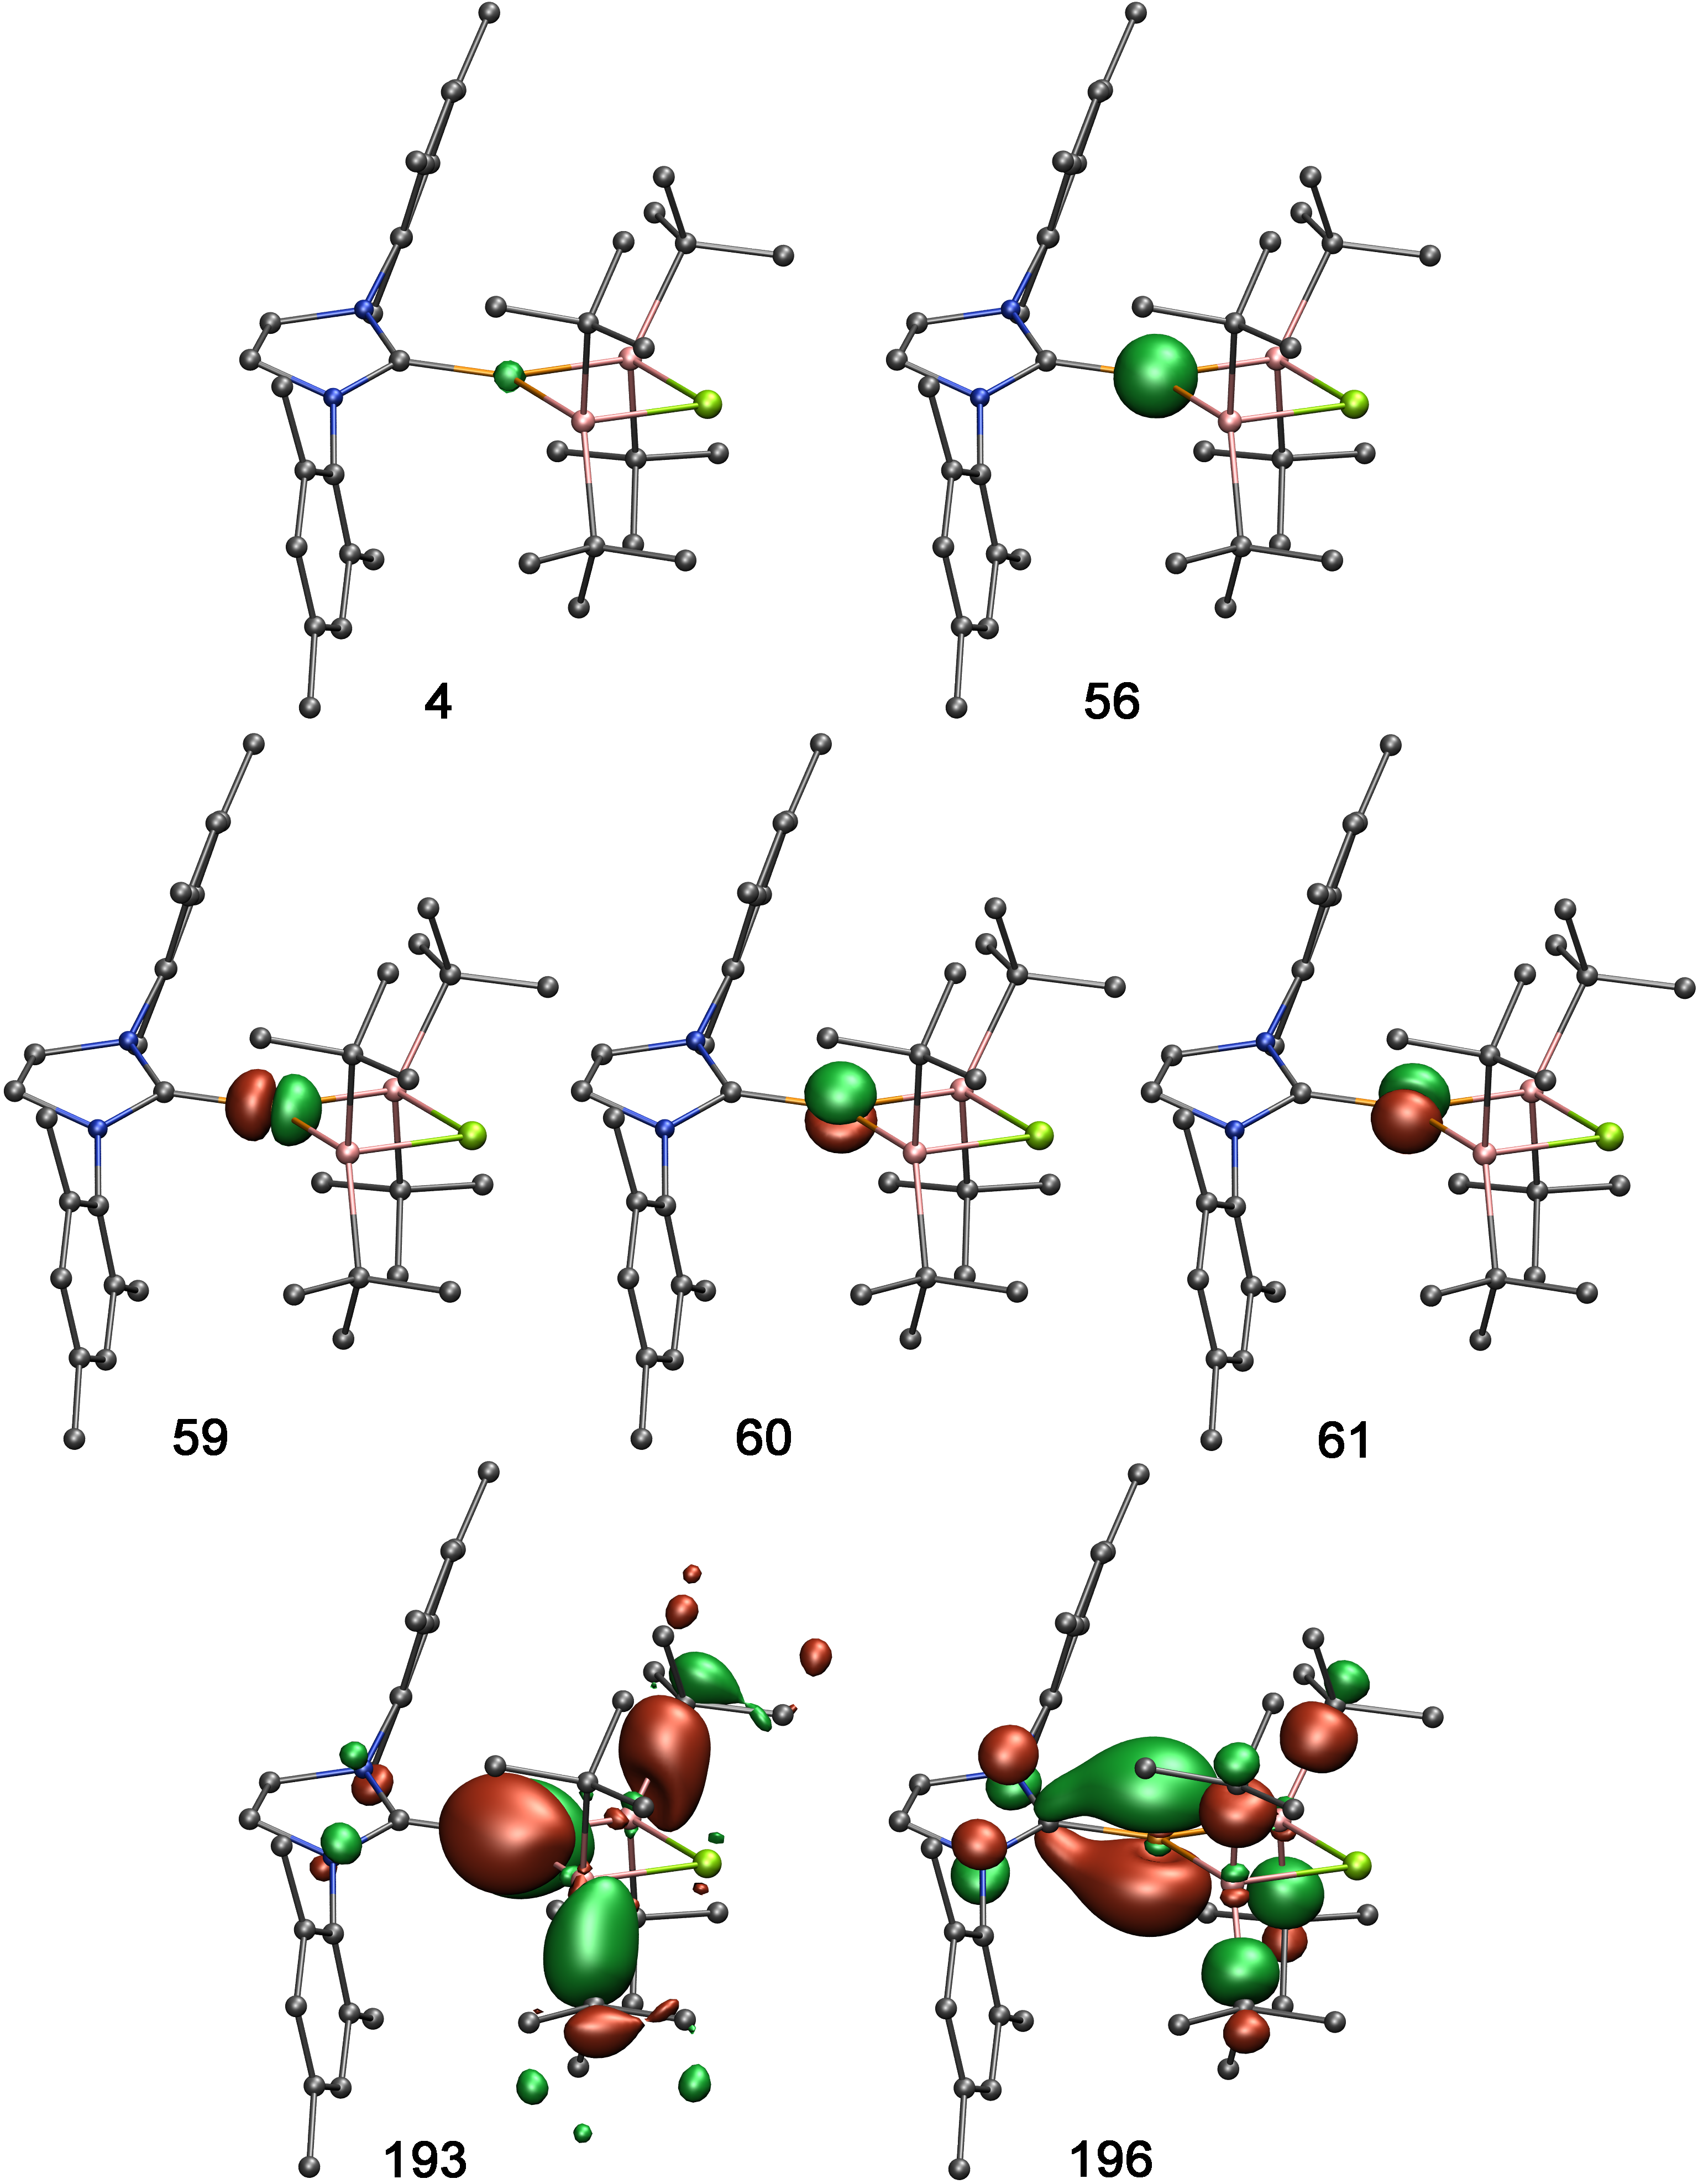
\includegraphics[width=1.0\textwidth]{modec}
	\captionsetup{figurewithin = chapter}
	\captionsetup{font=small, labelfont=bf}\caption[{Molekülorbitale von SIMesP(Ga\textit{t}Bu$_2$)$_2$Cl}]{Molekülorbitale mit den größten Beiträgen zur $^{31}$P Abschirmung in SIMesP(Ga\textit{t}Bu$_2$)$_2$Cl. Im einzelnen sind 4 das 1s, 56 das 2s und 59-61 die 2p Orbitale des Phosphors. 193 und 196 die C-P $\pi$-Orbitale. Gleichzeitig ist 196 auch das höchst besetzte \ac{mo} der Verbindung (Kohlenstoff=grau, Wasserstoff=weiß, Stickstoff=blau, Phosphor=orange, Gallium=rosa und Chlor=grün). Die Wasserstoffatome wurden zur besseren Veranschaulichung bei der Abbildung weg gelassen.}
\label{abb:modec}
\end{figure}